\documentclass[onecolumn,unpublished]{quantumarticle}
\usepackage{amsmath}
\usepackage{amssymb}
\usepackage{amsthm}
\usepackage{amsfonts}
\usepackage[caption=false]{subfig}
\usepackage[colorlinks]{hyperref}
\usepackage[all]{hypcap}
\usepackage{tikz}
\usepackage{relsize}
\usepackage{color,soul}
\usepackage[utf8]{inputenc}
\usepackage{capt-of}
\usepackage[numbers]{natbib}
\usetikzlibrary{decorations.pathreplacing}

% Boo Roman Numerals.
\renewcommand\thesection{\arabic{section}}

% Hyperlinked references to figures, theorems, etc.
\theoremstyle{definition}
\newtheorem{definition}{Definition}[section]
\theoremstyle{definition}
\newtheorem{theorem}[definition]{Theorem}
\theoremstyle{definition}
\newtheorem{lemma}[definition]{Lemma}
\newcommand{\eq}[1]{\hyperref[eq:#1]{Equation~\ref*{eq:#1}}}
\renewcommand{\sec}[1]{\hyperref[sec:#1]{Section~\ref*{sec:#1}}}
\DeclareRobustCommand{\app}[1]{\hyperref[app:#1]{Appendix~\ref*{app:#1}}}
\newcommand{\fig}[1]{\hyperref[fig:#1]{Figure~\ref*{fig:#1}}}
\newcommand{\tbl}[1]{\hyperref[tbl:#1]{Table~\ref*{tbl:#1}}}
\newcommand{\theoremref}[1]{\hyperref[theorem:#1]{Theorem~\ref*{theorem:#1}}}
\newcommand{\definitionref}[1]{\hyperref[definition:#1]{Definition~\ref*{definition:#1}}}

% Python style for highlighting
\usepackage{listings}
\DeclareFixedFont{\ttb}{T1}{txtt}{bx}{n}{12}
\DeclareFixedFont{\ttm}{T1}{txtt}{m}{n}{12}
\definecolor{deepblue}{rgb}{0,0,0.5}
\definecolor{deepred}{rgb}{0.6,0,0}
\definecolor{deepgreen}{rgb}{0,0.5,0}
\newcommand\pythonstyle{\lstset{
language=Python,
basicstyle=\ttm,
otherkeywords={self,controlledby,with,quint,let,carryinto,store},
keywordstyle=\ttb\color{deepblue},
emph={measure,__init__},
emphstyle=\ttb\color{deepblue},
stringstyle=\color{deepgreen},
showstringspaces=false
}}
\lstnewenvironment{python}[1][]
{\pythonstyle\lstset{#1}}{}

%    Q-circuit version 2
%    Copyright (C) 2004  Steve Flammia & Bryan Eastin
%    Last modified on: 9/16/2011
%
%    This program is free software; you can redistribute it and/or modify
%    it under the terms of the GNU General Public License as published by
%    the Free Software Foundation; either version 2 of the License, or
%    (at your option) any later version.
%
%    This program is distributed in the hope that it will be useful,
%    but WITHOUT ANY WARRANTY; without even the implied warranty of
%    MERCHANTABILITY or FITNESS FOR A PARTICULAR PURPOSE.  See the
%    GNU General Public License for more details.
%
%    You should have received a copy of the GNU General Public License
%    along with this program; if not, write to the Free Software
%    Foundation, Inc., 59 Temple Place, Suite 330, Boston, MA  02111-1307  USA

% Thanks to the Xy-pic guys, Kristoffer H Rose, Ross Moore, and Daniel Müllner,
% for their help in making Qcircuit work with Xy-pic version 3.8.  
% Thanks also to Dave Clader, Andrew Childs, Rafael Possignolo, Tyson Williams,
% Sergio Boixo, Cris Moore, Jonas Anderson, and Stephan Mertens for helping us test 
% and/or develop the new version.

\usepackage[color]{xy}
\UseCrayolaColors
\xyoption{matrix}
\xyoption{frame}
\xyoption{arrow}
\xyoption{arc}

\usepackage{ifpdf}
\ifpdf
\else
\PackageWarningNoLine{Qcircuit}{Qcircuit is loading in Postscript mode.  The Xy-pic options ps and dvips will be loaded.  If you wish to use other Postscript drivers for Xy-pic, you must modify the code in Qcircuit.tex}
%    The following options load the drivers most commonly required to
%    get proper Postscript output from Xy-pic.  Should these fail to work,
%    try replacing the following two lines with some of the other options
%    given in the Xy-pic reference manual.
\xyoption{ps}
\xyoption{dvips}
\fi

% The following resets Xy-pic matrix alignment to the pre-3.8 default, as
% required by Qcircuit.
\entrymodifiers={!C\entrybox}

%\newcommand{\bra}[1]{{\left\langle{#1}\right\vert}}
%\newcommand{\ket}[1]{{\left\vert{#1}\right\rangle}}
    % Defines Dirac notation. %7/5/07 added extra braces so that the commands will work in subscripts.
\newcommand{\qw}[1][-1]{\ar @{-} [0,#1]}
\newcommand{\eqw}[1][-1]{\ar @{-} @[Red] [0,#1]}
    % Defines a wire that connects horizontally.  By default it connects to the object on the left of the current object.
    % WARNING: Wire commands must appear after the gate in any given entry.
\newcommand{\qwx}[1][-1]{\ar @{-} [#1,0]}
    % Defines a wire that connects vertically.  By default it connects to the object above the current object.
    % WARNING: Wire commands must appear after the gate in any given entry.
\newcommand{\cw}[1][-1]{\ar @{=} [0,#1]}
    % Defines a classical wire that connects horizontally.  By default it connects to the object on the left of the current object.
    % WARNING: Wire commands must appear after the gate in any given entry.
\newcommand{\cwx}[1][-1]{\ar @{=} [#1,0]}
    % Defines a classical wire that connects vertically.  By default it connects to the object above the current object.
    % WARNING: Wire commands must appear after the gate in any given entry.
\newcommand{\gate}[1]{*+<.6em>{#1} \POS ="i","i"+UR;"i"+UL **\dir{-};"i"+DL **\dir{-};"i"+DR **\dir{-};"i"+UR **\dir{-},"i" \qw}
\newcommand{\eboxgate} [1]{*+<.6em>{#1} \POS ="i","i"+UR;"i"+UL **[red]\dir{-};"i"+DL **[red]\dir{-};"i"+DR **[red]\dir{-};"i"+UR **[red]\dir{-},"i" \eqw}
\newcommand{\circgate}[1]{*+<0.6em>[o][F-]{#1} \eqw}
\newcommand{\ecircgate}[1]{*+<0.6em>[o][F-:red]{#1} \eqw}
\newcommand{\filtergt}[1]{\eboxgate{\scriptscriptstyle{#1}}}
\newcommand{\idealdec}{*+<1.2em>{\phantom{*}} \POS ="i","i"+UL;"i"+DL **[red]\dir{-};"i"+R **[red]\dir{-};"i"+UL **[red]\dir{-},"i" \eqw}

    % Boxes the argument, making a gate.
\newcommand{\meter}{*=<1.8em,1.4em>{\xy ="j","j"-<.778em,.322em>;{"j"+<.778em,-.322em> \ellipse ur,_{}},"j"-<0em,.4em>;p+<.5em,.9em> **\dir{-},"j"+<2.2em,2.2em>*{},"j"-<2.2em,2.2em>*{} \endxy} \POS ="i","i"+UR;"i"+UL **\dir{-};"i"+DL **\dir{-};"i"+DR **\dir{-};"i"+UR **\dir{-},"i" \qw}
    % Inserts a measurement meter.
    % In case you're wondering, the constants .778em and .322em specify
    % one quarter of a circle with radius 1.1em.
    % The points added at + and - <2.2em,2.2em> are there to strech the
    % canvas, ensuring that the size is unaffected by erratic spacing issues
    % with the arc.
\newcommand{\measure}[1]{*+[F-:<.9em>]{#1} \qw}
    % Inserts a measurement bubble with user defined text.
\newcommand{\measuretab}[1]{*{\xy*+<.6em>{#1}="e";"e"+UL;"e"+UR **\dir{-};"e"+DR **\dir{-};"e"+DL **\dir{-};"e"+LC-<.5em,0em> **\dir{-};"e"+UL **\dir{-} \endxy} \qw}
    % Inserts a measurement tab with user defined text.
\newcommand{\measureD}[1]{*{\xy*+=<0em,.1em>{#1}="e";"e"+UR+<0em,.25em>;"e"+UL+<-.5em,.25em> **\dir{-};"e"+DL+<-.5em,-.25em> **\dir{-};"e"+DR+<0em,-.25em> **\dir{-};{"e"+UR+<0em,.25em>\ellipse^{}};"e"+C:,+(0,1)*{} \endxy} \qw}
\newcommand{\emeasureD}[1]{*{\xy*+=<0em,.1em>{#1}="e";"e"+UR+<0em,.25em>;"e"+UL+<-.5em,.25em> **[red]\dir{-};"e"+DL+<-.5em,-.25em> **[red]\dir{-};"e"+DR+<0em,-.25em> **[red]\dir{-};{"e"+UR+<0em,.25em>\ellipse{}};"e"+C:,+(0,1)*{} \endxy} \qw}
    % Inserts a D-shaped measurement gate with user defined text.
\newcommand{\multimeasure}[2]{*+<1em,.9em>{\hphantom{#2}} \qw \POS[0,0].[#1,0];p !C *{#2},p \drop\frm<.9em>{-}}
    % Draws a multiple qubit measurement bubble starting at the current position and spanning #1 additional gates below.
    % #2 gives the label for the gate.
    % You must use an argument of the same width as #2 in \ghost for the wires to connect properly on the lower lines.
\newcommand{\multimeasureD}[2]{*+<1em,.9em>{\hphantom{#2}} \POS [0,0]="i",[0,0].[#1,0]="e",!C *{#2},"e"+UR-<.8em,0em>;"e"+UL **\dir{-};"e"+DL **\dir{-};"e"+DR+<-.8em,0em> **\dir{-};{"e"+DR+<0em,.8em>\ellipse^{}};"e"+UR+<0em,-.8em> **\dir{-};{"e"+UR-<.8em,0em>\ellipse^{}},"i" \qw}
    % Draws a multiple qubit D-shaped measurement gate starting at the current position and spanning #1 additional gates below.
    % #2 gives the label for the gate.
    % You must use an argument of the same width as #2 in \ghost for the wires to connect properly on the lower lines.
\newcommand{\control}{*!<0em,.025em>-=-<.2em>{\bullet}}
    % Inserts an unconnected control.
\newcommand{\controlo}{*+<.01em>{\xy -<.095em>*\xycircle<.19em>{} \endxy}}
    % Inserts a unconnected control-on-0.
\newcommand{\ctrl}[1]{\control \qwx[#1] \qw}
    % Inserts a control and connects it to the object #1 wires below.
\newcommand{\ctrlo}[1]{\controlo \qwx[#1] \qw}
    % Inserts a control-on-0 and connects it to the object #1 wires below.
\newcommand{\targ}{*+<.02em,.02em>{\xy ="i","i"-<.39em,0em>;"i"+<.39em,0em> **\dir{-}, "i"-<0em,.39em>;"i"+<0em,.39em> **\dir{-},"i"*\xycircle<.4em>{} \endxy} \qw}
    % Inserts a CNOT target.
\newcommand{\qswap}{*=<0em>{\times} \qw}
    % Inserts half a swap gate.
    % Must be connected to the other swap with \qwx.
\newcommand{\multigate}[2]{*+<1em,.9em>{\hphantom{#2}} \POS [0,0]="i",[0,0].[#1,0]="e",!C *{#2},"e"+UR;"e"+UL **\dir{-};"e"+DL **\dir{-};"e"+DR **\dir{-};"e"+UR **\dir{-},"i" \qw}
    % Draws a multiple qubit gate starting at the current position and spanning #1 additional gates below.
    % #2 gives the label for the gate.
    % You must use an argument of the same width as #2 in \ghost for the wires to connect properly on the lower lines.
\newcommand{\ghost}[1]{*+<1em,.9em>{\hphantom{#1}} \qw}
    % Leaves space for \multigate on wires other than the one on which \multigate appears.  Without this command wires will cross your gate.
    % #1 should match the second argument in the corresponding \multigate.
\newcommand{\push}[1]{*{#1}}
    % Inserts #1, overriding the default that causes entries to have zero size.  This command takes the place of a gate.
    % Like a gate, it must precede any wire commands.
    % \push is useful for forcing columns apart.
    % NOTE: It might be useful to know that a gate is about 1.3 times the height of its contents.  I.e. \gate{M} is 1.3em tall.
    % WARNING: \push must appear before any wire commands and may not appear in an entry with a gate or label.
\newcommand{\gategroup}[6]{\POS"#1,#2"."#3,#2"."#1,#4"."#3,#4"!C*+<#5>\frm{#6}}
    % Constructs a box or bracket enclosing the square block spanning rows #1-#3 and columns=#2-#4.
    % The block is given a margin #5/2, so #5 should be a valid length.
    % #6 can take the following arguments -- or . or _\} or ^\} or \{ or \} or _) or ^) or ( or ) where the first two options yield dashed and
    % dotted boxes respectively, and the last eight options yield bottom, top, left, and right braces of the curly or normal variety.  See the Xy-pic reference manual for more options.
    % \gategroup can appear at the end of any gate entry, but it's good form to pick either the last entry or one of the corner gates.
    % BUG: \gategroup uses the four corner gates to determine the size of the bounding box.  Other gates may stick out of that box.  See \prop.

\newcommand{\rstick}[1]{*!L!<-.5em,0em>=<0em>{#1}}
    % Centers the left side of #1 in the cell.  Intended for lining up wire labels.  Note that non-gates have default size zero.
\newcommand{\lstick}[1]{*!R!<.5em,0em>=<0em>{#1}}
    % Centers the right side of #1 in the cell.  Intended for lining up wire labels.  Note that non-gates have default size zero.
\newcommand{\ustick}[1]{*!D!<0em,-.5em>=<0em>{#1}}
    % Centers the bottom of #1 in the cell.  Intended for lining up wire labels.  Note that non-gates have default size zero.
\newcommand{\dstick}[1]{*!U!<0em,.5em>=<0em>{#1}}
    % Centers the top of #1 in the cell.  Intended for lining up wire labels.  Note that non-gates have default size zero.
\newcommand{\Qcircuit}{\xymatrix @*=<0em>}
    % Defines \Qcircuit as an \xymatrix with entries of default size 0em.
\newcommand{\link}[2]{\ar @{-} [#1,#2]}
    % Draws a wire or connecting line to the element #1 rows down and #2 columns forward.
\newcommand{\pureghost}[1]{*+<1em,.9em>{\hphantom{#1}}}
    % Same as \ghost except it omits the wire leading to the left. 
%%%%%%%%%%%%%%%%%%%%%%%%%%%%%%%%%%%%%%%%%%%%%%%%%%%%%%%%%%%%%%%%%%%%%%%%%%%%%%%%%%%%%%%%%%
\newcommand{\multiprepareC}[2]{*+<1em,.9em>{\hphantom{#2}}\save[0,0].[#1,0];p\save !C
  *{#2},p+RU+<0em,0em>;+LU+<+.8em,0em> **\dir{-}\restore\save +RD;+RU **\dir{-}\restore\save
  +RD;+LD+<.8em,0em> **\dir{-} \restore\save +LD+<0em,.8em>;+LU-<0em,.8em> **\dir{-} \restore \POS
  !UL*!UL{\cir<.9em>{u_r}};!DL*!DL{\cir<.9em>{l_u}}\restore}
   % Draws a multiple qubit reverse-D-shaped preparation gate starting at the current position and spanning #1 additional gates below.
   % #2 gives the label for the gate.
   % You must use an argument of the same width as #2 in \pureghost for the wires to connect properly on
% the lower lines.
\newcommand{\prepareC}[1]{*{\xy*+=+<.5em>{\vphantom{#1\rule{0em}{.1em}}}*\cir{l^r};p\save*!L{#1} \restore\save+UC;+UC+<.5em,0em>*!L{\hphantom{#1}}+R **\dir{-} \restore\save+DC;+DC+<.5em,0em>*!L{\hphantom{#1}}+R **\dir{-} \restore\POS+UC+<.5em,0em>*!L{\hphantom{#1}}+R;+DC+<.5em,0em>*!L{\hphantom{#1}}+R **\dir{-} \endxy}}
   % Inserts a reverse-D-shaped preparation gate with user defined text.
\newcommand{\poloFantasmaCn}[1]{{{}^{#1}_{\phantom{#1}}}}


\title{Quantum lookahead adders and the wait for magic states}
\date{\today}
\author{Craig Gidney}
\email{craiggidney@google.com}
\affiliation{Google Inc., Santa Barbara, California 93117, USA}

\begin{document}
\maketitle

\begin{abstract}
We improve the Toffoli count of quantum lookahead adders, and analyze how their spacetime cost reacts to having a limited number of magic state factories.
We present an out-of-place carry lookahead adder with a Toffoli count of $4n$ (vs $5n$ in previous work by Draper et al) and a corresponding in-place Toffoli count of $7n$ (vs $10n$ in previous work by Draper et al).
We also present a block lookahead adder, that operates across blocks of bits of size $b$ and reduces the Toffoli count to $3n + 5n/b$ out-of-place and $5n + 5n/b$ in-place at the cost of the reaction depth depending linearly on $b$.
We estimate the spacetime volume of these adders, and adders from previous work, for various register sizes and factory counts under plausible assumptions for a large scale quantum computer based on the surface code and superconducting qubits.
\end{abstract}

\section{Introduction}

In the classical computing world, low depth adders are everywhere.
Even the original 8-bit Intel 8008 chip had a carry-lookahead adder \cite{shirriff2020reverseengineer8008}.
But it's not clear if low depth adders will enjoy the same popularity in the world of fault tolerant quantum computation, because of huge implied space overheads from magic state distillation.

The surface code \cite{fowler2012surfacereview} is a leading contender for the error correcting code used by future large scale quantum computers, because it has a high threshold and low connectivity requirements.
In the surface code, non-Clifford operations like the T gate and the Toffoli gate aren't native operations.
They have to be emulated using roundabout techniques like magic state distillation \cite{bravyi2005magicstate}.
Magic state factories are expected to be expensive.
For example in \cite{gidney2019catalyzed} a factory covers hundreds of thousands of physical qubits (although new techniques are reducing the cost \cite{litinski2019magicnotcostly}).

If a quantum computer can't host enough magic state factories, a low depth adder will bottleneck waiting for magic states.
Suppose we have a quantum computer with a control system reaction time of 10 microseconds and a factory design that produces a Toffoli state roughly every 165 microseconds as in \cite{gidney2019autoccz}.
Using a ripple-carry adder and reaction limited quantum computation \cite{fowler2012timeoptimal,gidney2019autoccz}, we would need 17 magic state factories before the ripple carry process was running at top speed.
If a low depth adder takes five times more Toffolis, we need five times more factories ($17 \cdot 5 = 85$) to compensate.
Ultimately this implies that, if we can't dedicate tens of millions of physical qubits to magic state distillation, the ripple carry adder will be faster by default.

\begin{table}
\centering
\resizebox{\linewidth}{!}{
\begin{tabular}{r|c|c|l|l|l|c|c|c|c}
Paper                                                &Place &Type                   &Toffolis                    &Reaction Depth             &Workspace                  &u    &V(n=100,f=10) &V(n=1000,f=100) &V(n=10000,f=1000) \\
\hline
Draper et al. (2004) \cite{draper2004lookaheadadder} &in    &Carry Lookahead        &$10n - 6\lg n - 13$         &$4\lg n + 7$               &$2n - \lg n - 1$           &1    &17            &180             &1800              \\
(this paper) (2020)                                  &in    &Carry Lookahead        &$7n$                        &$4\lg n + O(1)$            &$4n + O(1)$                &1    &15            &150             &1500              \\
(this paper) (2020)                                  &in    &b Blocks               &$5n + 10\frac{n}{b} + O(1)$ &$0\lg \frac{n}{b} + O(1)$  &$2n + 5\frac{n}{b} + O(1)$ &1    &3             &100             &1000              \\
(this paper) (2020)                                  &in    &Sqrt Blocks            &$5n + 6\sqrt n + O(1)$      &$6\sqrt n + 4\lg n + O(1)$ &$2n + 5\sqrt n + O(1)$     &1    &11            &97              &930               \\
(this paper) (2020)                                  &in    &Two Blocks             &$3n$                        &$1.5n + O(1)$              &$n$                        &0.75 &5             &80              &4800              \\
Cuccaro (2004) \cite{cuccaro2004adder}               &in    &Ripple Carry           &$2n - 1$                    &$2n - 1$                   &$1$                        &1    &3             &63              &4200              \\
Gidney (2017) \cite{gidney2018halving}               &in    &Ripple Carry           &$n - 1$                     &$2n - 1$                   &$n$                        &0.5  &2             &71              &6100              \\

\hline
Gossett (1998) \cite{gossett1998carrysave}           &out   &Pipelined (n summands) &$4n$                        &$2$                        &$n^2 - 2n$                 &1    &71            &6600            &660000            \\
Draper et al. (2004) \cite{draper2004lookaheadadder} &out   &Carry Lookahead        &$5n - 3\lg n - 4$           &$2\lg n + 3$               &$n - \lg n$                &1    &8             &91              &920               \\
(this paper) (2020)                                  &out   &Carry Lookahead        &$4n$                        &$2\lg n + O(1)$            &$3n + O(1)$                &1    &8             &87              &870               \\
(this paper) (2020)                                  &out   &b Blocks               &$3n + 5\frac{n}{b} + O(1)$  &$0\lg \frac{n}{b} + O(1)$  &$2n + 5\frac{n}{b} + O(1)$ &1    &2             &100             &1000              \\
(this paper) (2020)                                  &out   &Sqrt Blocks            &$3n + 3\sqrt n + O(1)$      &$3\sqrt n + 2\lg n + O(1)$ &$2n + 5\sqrt n + O(1)$     &1    &7             &63              &610               \\
Gidney (2017) \cite{gidney2018halving}               &out   &Ripple Carry           &$n - 1$                     &$n - 1$                    &$1$                        &1    &1             &41              &3100              \\
(this paper) (2020)                                  &out   &Two Blocks             &$2n$                        &$n + O(1)$                 &$n$                        &0.67 &4             &64              &4200              \\
\end{tabular}

}
    \caption{Comparison of various adders.
    The Toffoli over time column shows how many Toffolis a circuit executes during each time step (blank areas are due to AND uncomputations), using a logarithmic scale.
    The value $V(n,f)$ is an estimate (in units of logical qubits times seconds) of the spacetime volume required to execute an $n$-bit adder using at most $f$ magic state factories (see \sec{estimate} for more details).
    Generated by \texttt{assets/comparison\_table.py}.
    }
    \label{tbl:comparison}
\end{table}

\begin{figure}
    \centering
    \minipage{0.5\textwidth}
    \resizebox{\linewidth}{!}{
    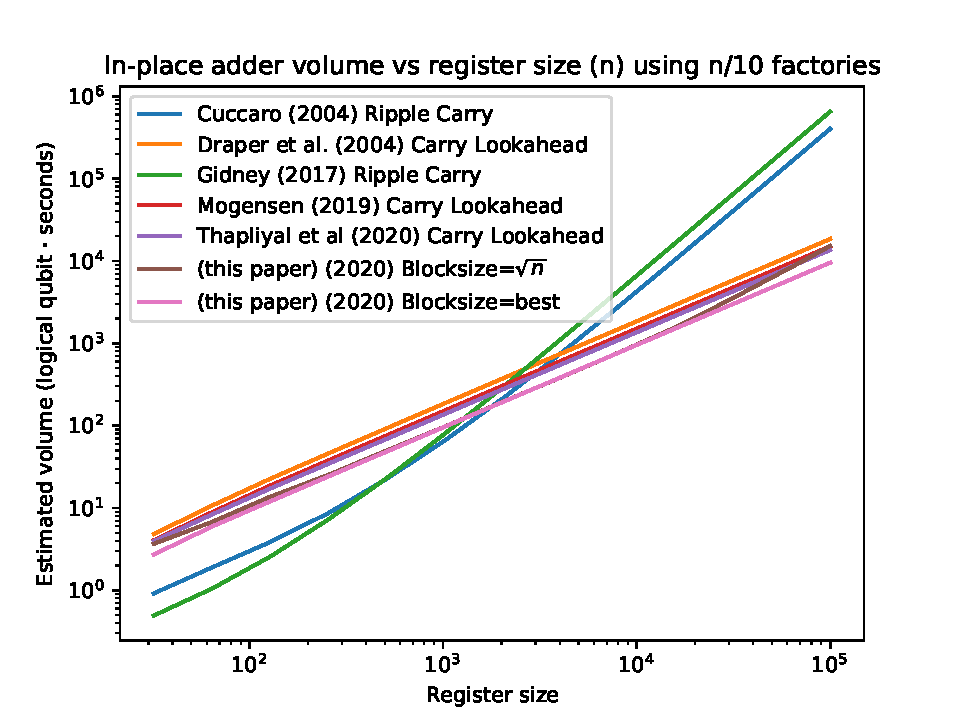
\includegraphics{gen/in-place-size-vs-vol.pdf}
    }
    \endminipage
    \minipage{0.5\textwidth}
    \resizebox{\linewidth}{!}{
    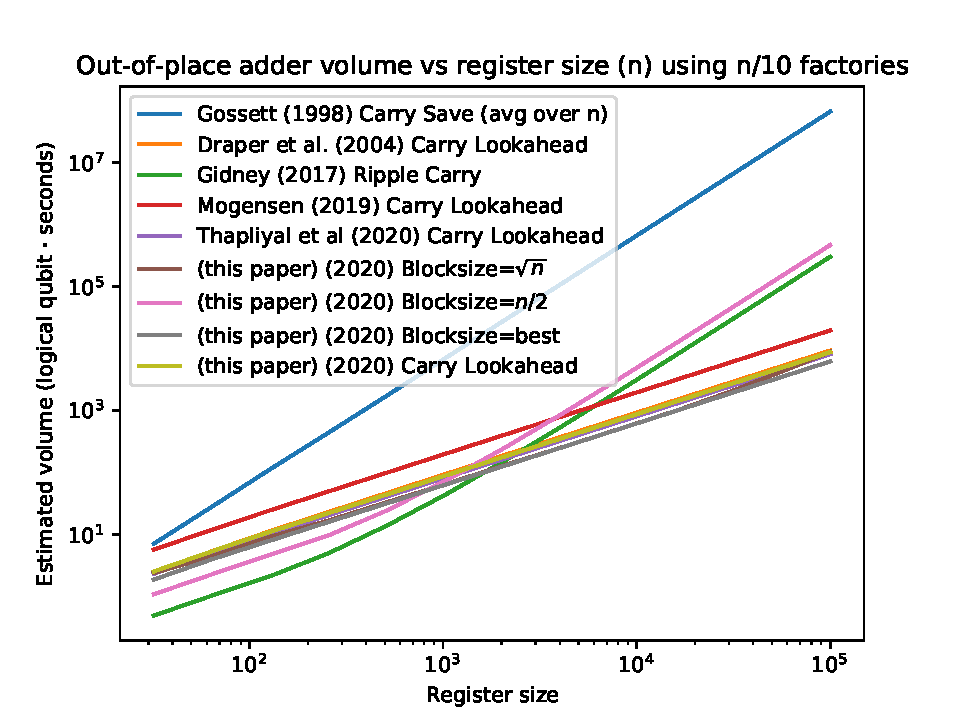
\includegraphics{gen/out-of-place-size-vs-vol.pdf}
    }
    \endminipage
    \caption{
        Log-log plot of adder spacetime volume versus register size. Assumes the maximum factory count is one tenth the register size, that factories have a footprint of 72 logical qubits, that factories produce a magic state every 165 microseconds, and that the control system reaction time is 10 microseconds.
        Generated by \texttt{assets/comparison\_table.py}.
    }
    \label{fig:size_versus_volume}
\end{figure}

\begin{figure}
    \centering
    \resizebox{\linewidth}{!}{
    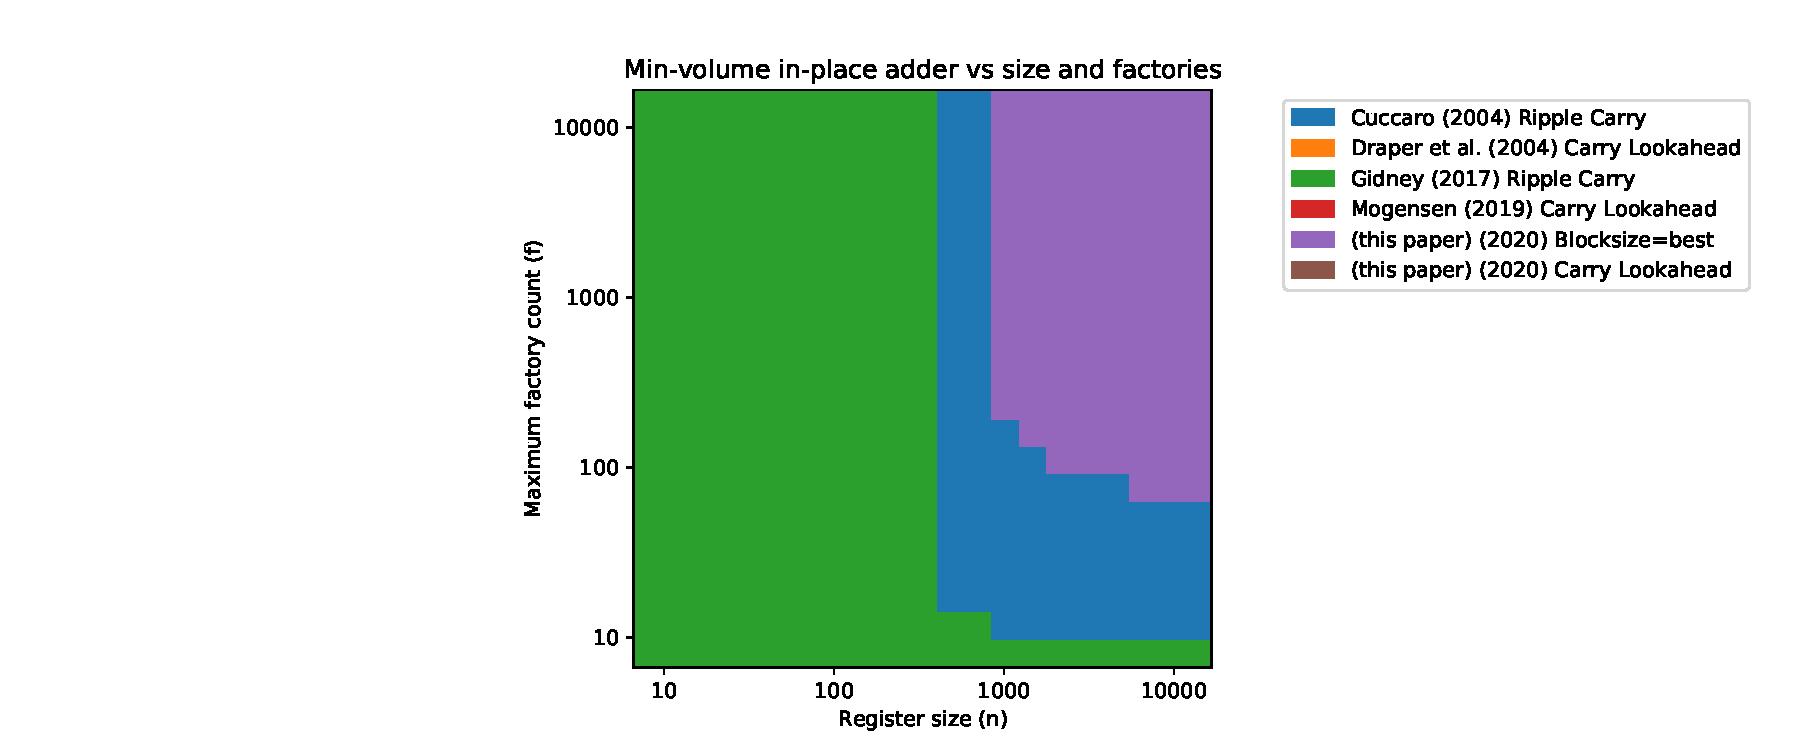
\includegraphics{gen/in-place-min-vol.pdf}
    }
    \caption{
        Lowest volume in-place adder at various register sizes and maximum factory counts.
        Assumes that factories have a footprint of 72 logical qubits, that factories produce a magic state every 165 microseconds, and that the control system reaction time is 10 microseconds.
        Generated by \texttt{assets/comparison\_table.py}.
    }
    \label{fig:minif}
\end{figure}

\begin{figure}
    \centering
    \resizebox{\linewidth}{!}{
    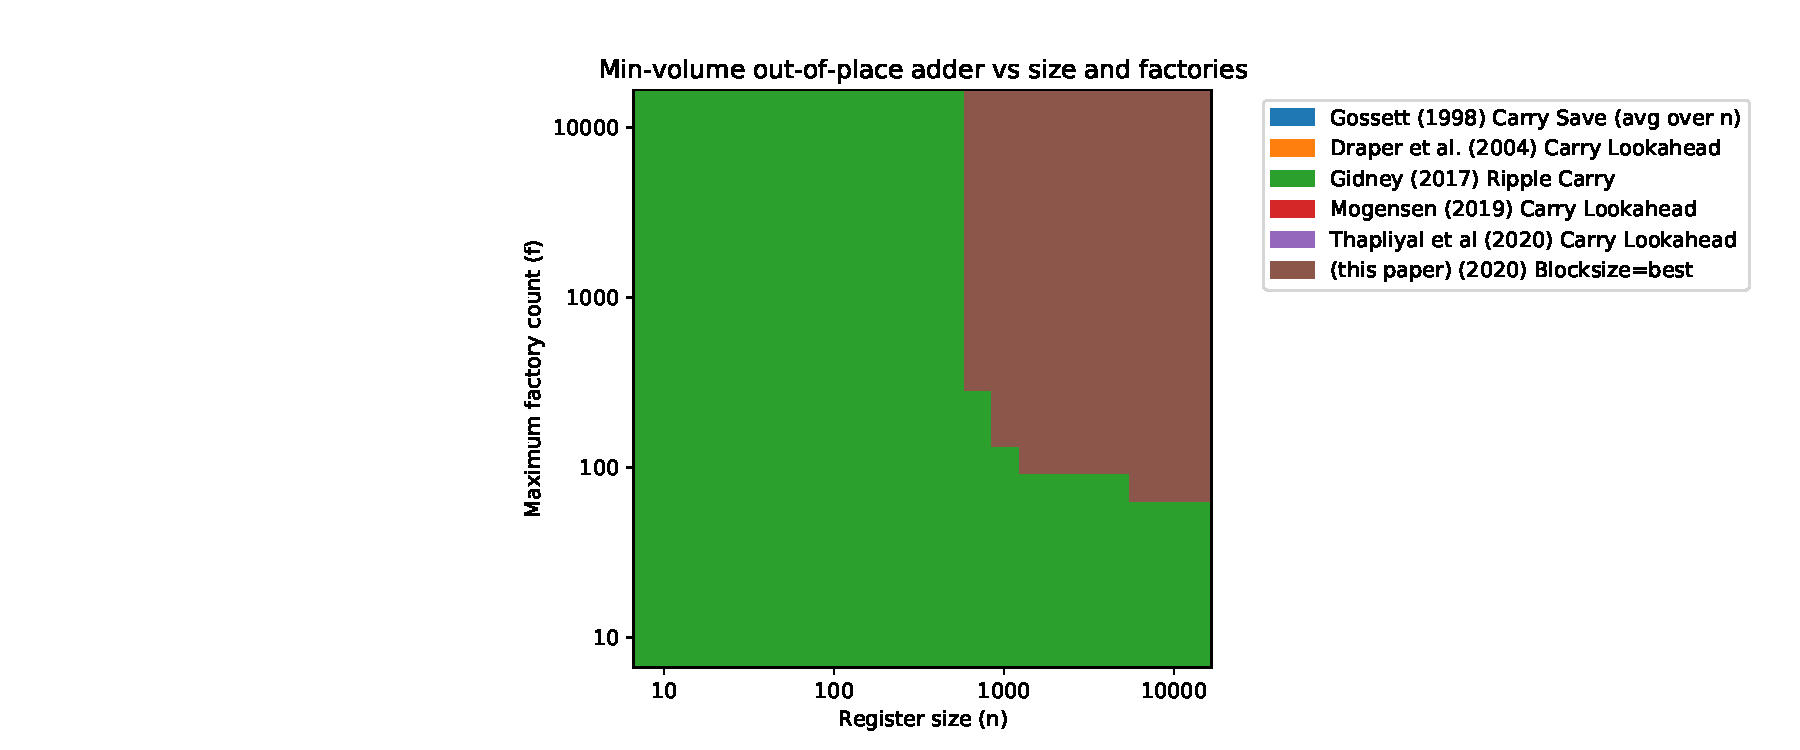
\includegraphics{gen/out-of-place-min-vol.pdf}
    }
    \caption{
        Lowest volume out-of-place adder at various register sizes and maximum factory counts.
        Assumes that factories have a footprint of 72 logical qubits, that factories produce a magic state every 165 microseconds, and that the control system reaction time is 10 microseconds.
        Generated by \texttt{assets/comparison\_table.py}.
    }
    \label{fig:minof}
\end{figure}

\begin{figure}
    \centering
    \resizebox{\linewidth}{!}{
    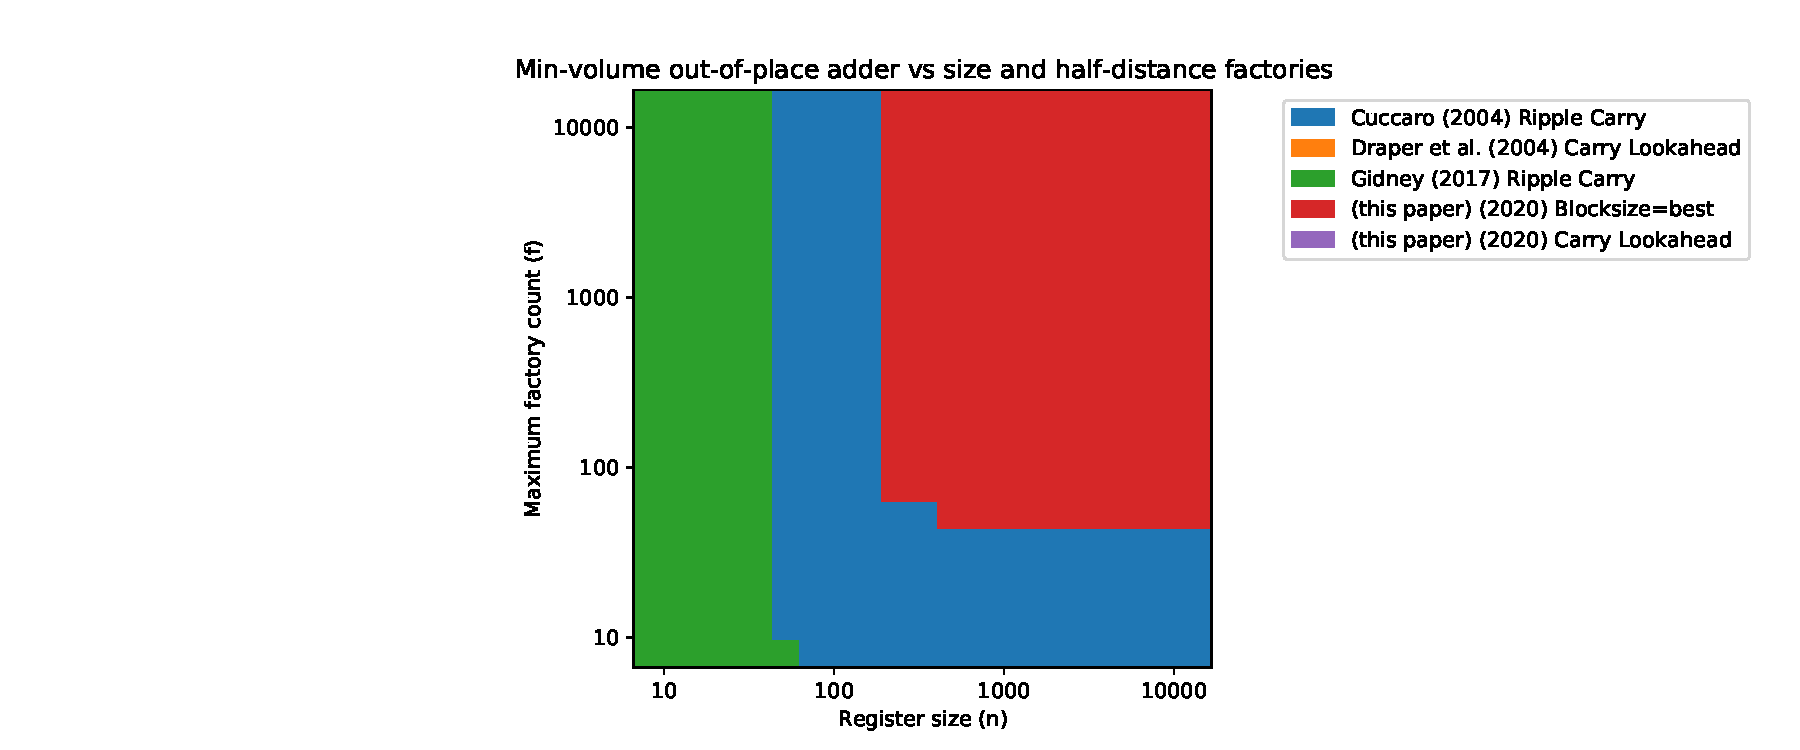
\includegraphics{gen/in-place-min-vol-half.pdf}
    }
    \resizebox{\linewidth}{!}{
    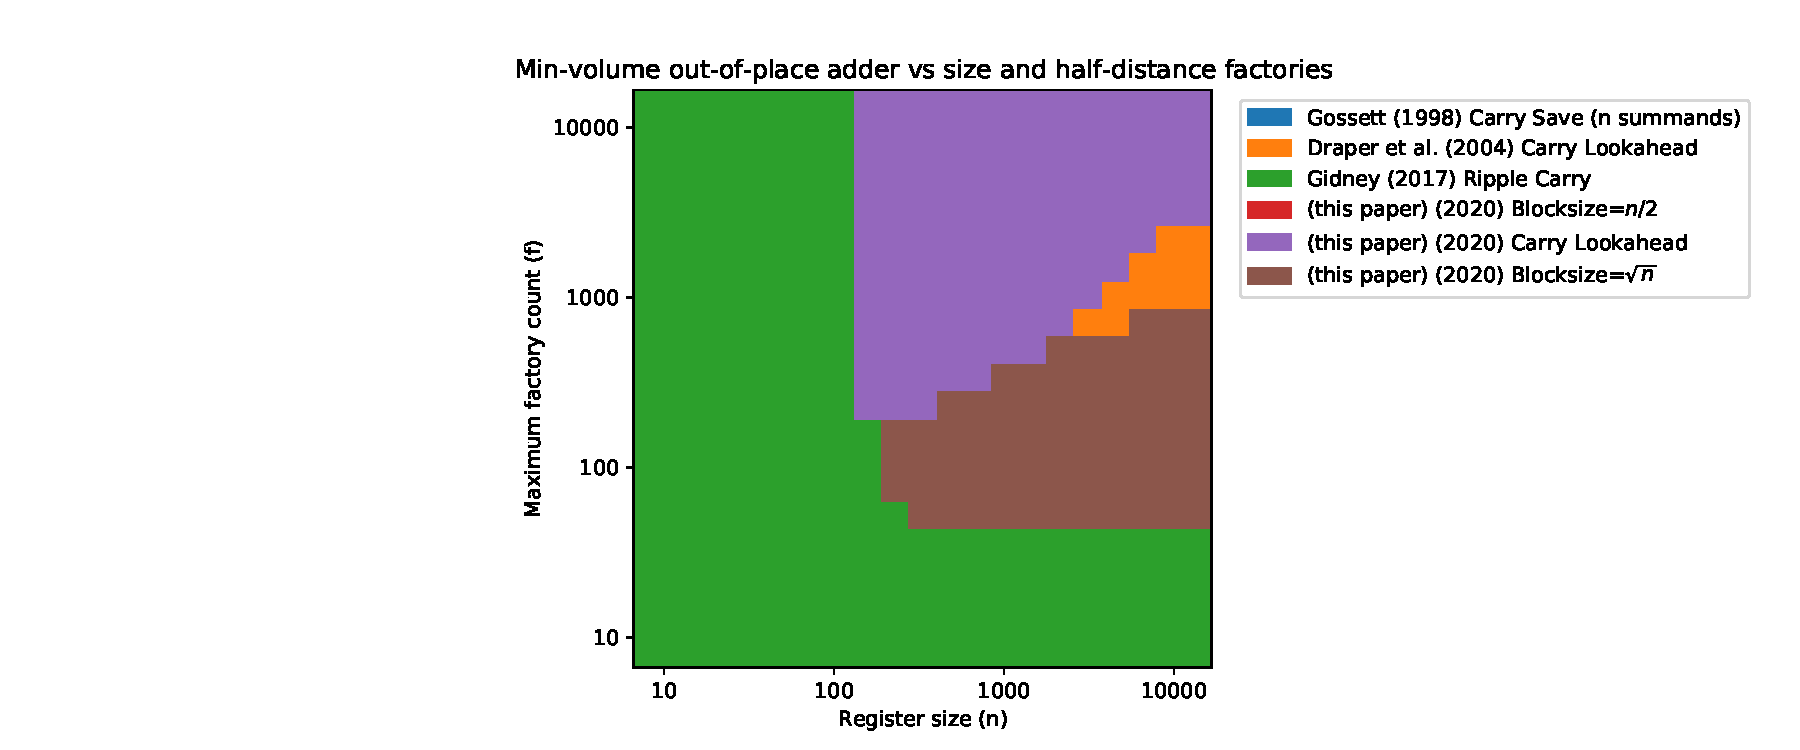
\includegraphics{gen/out-of-place-min-vol-half.pdf}
    }
    \caption{
        Lowest volume in-place and out-of-place adders at various register sizes and maximum factory counts, assuming improved magic state factories.
        Assumes that factories have a footprint of 18 logical qubits, that factories produce a magic state every 82.5 microseconds, and that the control system reaction time is 10 microseconds.
        Generated by \texttt{assets/comparison\_table.py}.
    }
    \label{fig:minioh}
\end{figure}

Although the example we just gave is in terms of the execution time of a circuit, focusing on just time can be misleading.
In this paper, we're going to focus on the spacetime volume consumed by a circuit instead.
This choice is based on the idea that any volume not used for one thing can be repurposed for some other useful task (like magic state distillation or temporary storage).
The topological nature of surface code computations, which allows for deformations and rotations through spacetime, makes this assumption better than it might seem.
That being said, beware that there are regimes where focusing on spacetime volume is the wrong thing to do.
For example, in a world where space is limitless, making magic state factories effectively free, time is king and low depth adders are almost trivially better than ripple carry adders.
But that is not the parameter regime we are interested in, so we will focus on volume.

Our goal in this paper is to reduce and quantify the spacetime overhead implicit in using a low depth adder.
We start in \sec{lookahead} by constructing a new carry lookahead adder based on quantizing the classical Brent-Kung adder \cite{brent1982adder} and on using temporary ANDs \cite{gidney2018halving}.
Then, in \sec{block}, we sacrifice parallelism to further lower the Toffoli overhead.
Instead of operating on every bit in parallel, we split the problem into blocks and operate on the blocks in parallel.
In \sec{estimate}, we estimate the spacetime volume of our adders and previous adders in order to understand the parameter regimes where various adders dominate.
Finally, in \sec{conclusion}, we summarize our results and give some additional caveats.


\section{Carry Lookahead Adder}
\label{sec:lookahead}

The Brent-Kung adder \cite{brent1982adder} is a classical binary adder circuit.
It achieves a logarithmic depth with fewer gates than comparable adders such as the Kogge-Stone adder \cite{kogge1973adder}.
The original motivating idea for this paper was to attempt to quantize the Brent-Kung adder.
The result is similar to the carry lookahead circuit created by Draper et al \cite{draper2004lookaheadadder}, with a key difference being the usage of additional ancilla to uncompute ANDs using no Toffoli gates \cite{gidney2018halving}.

To propagate carries quickly, we will be considering various contiguous bit ranges and computing a ternary value that describes the carry behavior of these ranges.
Define the integer bit slicing operation $k[a:b] = \lfloor k/2^a \rfloor \bmod 2^{b-a+1}$.
Let $x$ and $y$ be $n$-bit little-endian 2s-complement inputs into the addition.
We define

$$C_a^b = \text{median}(0, 2, x[a:b] + y[a:b] - 2^{b - a + 1} + 1)$$

If $C_a^b = 0$, that means the input bits in the range from $a$ to $b$ will produce a carry-out bit equal to 0 no matter what carry-in bit enters into the range.
If $C_a^b = 2$, the carry-out bit is guaranteed to be 1 regardless of the carry-in bit.
If $C_a^b = 1$, the carry-out bit will equal the carry-in bit.

Given a bit position, the ternary carry value describing the range from that bit position to the next bit position can be computed like this:

$$\text{unit\_carry}(a) = C_a^{a+1} = (x_a \land y_a) + 2 (x_a \oplus y_a)$$

Note that the 1s bit and the 2s bit of the carry value are computed independently, and that it would take one Toffoli operation to compute the pair of bits.

Ternary carry values whose range start and range end are equal can be fused together:

$$\text{fuse\_carry}(C_a^b, C_b^c) = C_a^c = \begin{cases}
C_b^c = 1 & \rightarrow C_a^b \\
C_b^c \neq 1 & \rightarrow C_b^c
\end{cases}$$

This computation can be performed using two Toffoli operations.
If only the 2s bit is needed (e.g. because the carry-in bit is known to be zero when the range starts at zero), only one Toffoli operation is needed.

The purpose of creating and fusing carry values together is to discover whether or not $C_0^k = 2$ for each bit position $k$.
This is useful because it tells us whether the bit in the sum at position $k$ should agree or disagree with the parity of $x$ and $y$ at position $k$.
That is to say:

$$(x + y)_k = x_k \oplus y_k \oplus (C_0^k = 2)$$

The main difficulty is in finding a good strategy for fusing carry values, that can perform many fusion steps in parallel but doesn't do too many fusion steps overall.
This is where the Brent-Kung adder comes in: it specifies a fusing pattern that we mimic.

We start by computing all unit length ranges $C_k^{k+1}$ in parallel, and then spend $\lg n + O(1)$ rounds iteratively fusing these ranges together to produce ranges that cross larger distances.
During round $s$, starting with $s=1$, we (in parallel) consider each bit position $k$ and fuse ranges of the form $C_{2^s 2k}^{2^s (k+1/2)}, C_{2^s (k+1/2) }^{2^s (k+1)}$.
We skip any ranges whose end falls beyond the end of the register.

Once the process of computing the carry values for long distances ranges has completed, we begin using those values to complete the carry values for ranges starting at 0.
Let $p$ be the largest power of two no larger than $n$.
We have already computed $C_{0,p}$ and $C_{p,p+p/2}$, and we can fuse these two carry values to get $C_{0,p+p/2}$.
We continue this process in rounds, where in round $s$ we fuse range pairs of the form $C_0^{p/2^s \cdot k}, C_{p/2^s \cdot k}^{p/2^s \cdot k+p/2^{s+1}}$ and end up knowing all values $C_{0}^{k}$ where $k$ is a multiple of $p/2^{s+1}$.
After $\lg n + O(1)$ rounds we know all of the carry-from-zero values, and can compute the final sum.
All that's left to do is to uncompute the intermediate carry values.

This process is implemented by the \texttt{init\_sum\_using\_carry\_lookahead} method in the \\\texttt{src/adder\_lookahead.qs} ancillary file.

The method as described has a Toffoli cost of $4n$.
This can be somewhat easily seen in the Q\# code, because the only Toffoli operations are \texttt{init\_and} operations initializing the contents of four registers each of size $n$.
The four registers are storing the 2s bits of the carry values for the initial unit length ranges (the 1s bits are temporarily stored in-place over one of the inputs), the 1s bits and 2s bits of the carry values created while growing the carry value ranges, and the final propagated carry values.

The reaction depth of the method is $2 \lg n  + O(1)$.
The first $\lg n$ comes from growing the ranges.
The remaining $\lg n + O(1)$ comes from using the grown ranges to find zero-rooted ranges, and uncomputing the grown range values in parallel with this step.
(The uncomputation can happen in parallel because the grown range values are used in reverse order while computing the zero-rooted ranges.)

\begin{figure}
\centering
\resizebox{0.85\linewidth}{!}{
\Qcircuit @R=1em @C=0.75em {
\\
&{/} \qw& \ustick{n}\qw&\gate{\text{input }a}     &\qw       &\qw       &\gate{\text{input }a}              &\qw       &\qw& & & & & & &{/} \qw& \ustick{n}\qw&\qw&\gate{\text{input }a}&\qw&\\
&{/} \qw& \ustick{n}\qw&\gate{\text{input }b} \qwx&\qswap    &\gate{X}  &\gate{\text{input }b}          \qwx&\gate{X}  &\qw& & &=& & & &{/} \qw& \ustick{n}\qw&\qw&\gate{\text{+}a}\qwx&\qw&\\
\lstick{|0\rangle^{\otimes n}}&{/} \qw& \ustick{n}\qw&\gate{\text{init }a+b}\qwx&\qswap\qwx&\gate{X}  &\gate{(\text{init }a+b)^\dagger}\qwx&\qw       &\qw&&&&\lstick{|0\rangle^{\otimes n}}& & & & & & & & \\
\\
}
}
    \caption{
        Converting an out-of-place adder into an in-place adder by running the out-of-place adder forwards and then backwards, with a few additional swap and Pauli operations.
        Swap and Pauli operations can be tracked within the classical control system instead of actually being applied to the qubits.
    }
    \label{fig:oop2ip}
\end{figure}

In order to convert this out-of-place adder into an in-place adder, we use the construction shown in \fig{oop2ip}.
This runs the out-of-place adder forwards, and then backwards, with no other notable cost.
Three allocated registers were uncomputed when computing the out-of-place sum.
When running the out-of-place sum backwards, these registers will be recomputed costing $3n$ Toffolis.
Therefore the resulting in-place adder has a total Toffoli count of $7n$, a doubled reaction depth of $4 \lg n + O(1)$, and the same workspace cost of $3n$.
(The Toffoli count is $7n$ instead of $8n$ because the backwards process is not recomputing the propagated carry bits; it is uncomputing them.)

\section{Block Lookahead Adder}
\label{sec:block}

In the previous section we computed an initial carry value for every bit position, and then began combining these carry values.
We can instead start the process by computing initial carry values for blocks of $b$ bits.
To give a sense of how this will work, we start with a minimally-parallel parallel adder: the two block adder.
It divides an $n$-bit addition problem into two $n/2$-bit chunks and performs three ripple carry additions in parallel: adding the low chunks with no carry input, adding the high chunks with no carry input, and adding the high chunks with a set carry input.
As soon as the low chunk addition produces a carry output, this carry output is used to decide which of the two high chunk addition results to keep, and then intermediate values are uncomputed.

Here is pseudo-code describing the two block adder:

\begin{python}
    # Parallel ripple-carry adders.
    let out_low = a_low + b_low carryinto carry_out
    let case0 = a_high + b_high
    let case1 = a_high + b_high + 1
    # Choose high result using carry_out from low half.
    let out_high = case0 if carry_out else case1
    # Uncompute intermediate values in parallel.
    del carry_out
    del case1
    del case0
\end{python}

The ancillary file \texttt{src/adder\_two\_block.qs} has Q\# code implementing this adder.

We can generalize the two  block adder into an adder with $m$ blocks, or equivalently into an adder with blocks of width $b$ where $m=n/b$.
We can use the carry-fusing subroutine we created in the previous section to quickly propagate carry values between these blocks, and use the propagated carry value to keep the correct output from each block.
The main cost we pay for doing this, compared to parallelizing over every bit, is that the 1s bit of the initial carry values is no longer the xor of the two inputs.
We will need to spend Toffolis computing these bits and allocate a register to storing them.
Fortunately, the benefits we gain will outweigh these costs.

The Toffoli count of the block lookahead adder depends on both the register size $n$ and the block size $b$.
To start with, there are $2n-b$ Toffolis used to compute the two carry-in cases for each block except the first block.
The carry-out bits of these cases are combined into initial ternary carry values, and $3n/b$ Toffolis are used to compute final propagated carry values from these initial values.
Once the final propagated carry values are available, $n-b$ Toffolis are used to control, for each block except the first block, which of the carry-in cases is kept.
Then all intermediate values are uncomputed using no Toffolis.

The total Toffoli count of this out-of-place adder is $3n + 5n/b$, which is less than the adder from the previous section as long as $b > 5$.
The number of work qubits is also lower when $b > 5$.
The tradeoff is that the depth now depends linearly on $b$, because of the ripple carry adders used to compute (and uncompute) the initial block carry values.

This process is implemented by the \texttt{init\_sum\_using\_blocks} method in the \\\texttt{src/adder\_blocks.qs} ancillary file.


\section{Comparison}
\label{sec:estimate}

In a tiny quantum computer that can barely support a single magic state factory, ripple carry adders will always be best.
Conversely, in a huge quantum computer where space is too cheap to meter, low depth adders will dominate.
In this section our goal is to understand the intermediate regime between these two extremes.
Beware that some architectural parameters can have surprising effects.
For example, slowing down the physical qubits used by a quantum computer will decrease (not increase!) the effectiveness of low depth adders.
This happens because architectures with slower physical qubits have a larger ratio $r$ between the reaction time of the control system and the depth of a magic state factory.
They can do more control system round trips per factory, meaning reaction-limited computation can feed the outputs of more factories into a single serial circuit.

To compare adders, we started by looking up or computing their Toffoli count, reaction depth, workspace, and Toffoli consumption rates over time.
The Toffoli count is the number of Toffoli magic states that the circuit would consume.
The reaction depth is the deepest chain of sequential adaptive measurements that occur in the circuit (keeping in mind that in the surface code every Toffoli gate, AND computation, and AND uncomputation involves an adaptive measurement).
The workspace is the number of additional logical qubits needed in the abstract circuit model to run the circuit (i.e. not counting logical qubits used for magic state factories or for storing the input/output).
These values are listed in \tbl{comparison}.

With the adder data collected, we wrote code to estimate the spacetime volume of an adder given a specified reaction time, factory footprint, and factory period.
The code can be found in the \texttt{vol} method of the \texttt{Adder} class in the ancillary file \texttt{src/comparison\_table.py}.
The code adds together spacetime estimates for the distillation of Toffoli states needed by the circuit, for storage of the circuit's input and output data, for storage of temporary qubits allocated during the execution of the circuit, and for buffering magic states during low-Toffoli-consumption periods in the circuit.
If an adder needed fewer factories than the maximum, we did not count the unused factories against its spacetime volume (i.e. we assumed they would be used for something else instead).

We used the volume estimation code to generate several figures.
\fig{size_versus_volume} plots the estimated spacetime volume of an adder versus the register size of the addition being performed, assuming the maximum factory count is 10\% of the register size.
Note how, in this figure, the best adders are ripple-carry adders until register sizes are in the thousands.
In \fig{minif} and \fig{minof} we plotted 2d heatmaps showing the in-place and out-of-place adders with the best estimated spacetime volume, for various register sizes and maximum factory counts.
Once again the best adders are ripple-carry adders until register sizes are in the thousands, but this plot also shows that ripple carry adders dominate until factory counts are nearly 100.
\fig{minioh} also has 2d heatmaps showing the adder with the best estimated spacetime volume, but assumes improved factories using half the code distance (i.e. a quarter the footprint area and half the duration).
This moves the transition from ripple-carry adders to lookahead adders downwards, to register sizes in the hundreds of qubits and factory counts around 50.

\section{Conclusion}
\label{sec:conclusion}

In this paper we presented a carry lookahead adder with a lower Toffoli count than in previous work, and a block lookahead adder that can further lower the Toffoli count at the cost of increasing the depth.
We implemented these adders in Q\#, which allowed us to verify that they computed the correct result while using at most the stated number of Toffolis and workspace qubits (unfortunately Q\# is not currently able to verify the reaction depth).
We wrote Python code to estimate the spacetime volume of these adders, and previous adders, and compared them over a range of register sizes and maximum factory counts.
We found that our adders have lower spacetime volume than previous low depth adders.
However, we also demonstrated that ripply carry adders have the best estimated spacetime volumes for register sizes up to 200 and for maximum factory counts up to 50.
This is a surprising contrast to the classical world, where carry lookahead adders are used even for 8 bit additions \cite{shirriff2020reverseengineer8008}.

An important type of adder that we didn't consider in this paper is adders that operate on representations of an integer other than 2s complement.
These adders cannot be used in all situations, but are sometimes the best choice.
For example, consider that Shor's factoring algorithm \cite{shor1994algorithms} seems to be a perfect candidate for carry lookahead adders because Shor's factoring algorithm perform arithmetic on registers whose sizes are in the thousands.
However, by adding log-sized ``carry runways" to registers, the addition problem can be split into (an exponentially good approximation of) independent pieces \cite{gidney2019approximate}.
Also, it's possible to stay in this format while executing Shor's algorithm \cite{gidney2019factor}.
This means that parallelization of the additions in Shor's algorithm can be done with additive logarithmic overhead in the Toffoli count (via carry runways) instead of constant multiplicative overhead (via carry lookahead).

Overall, we believe that a clear conclusion of our work and our numerics is that quantum lookahead adders are rarely the best choice of adder.
At least, not in our cost model; which we think is representative of potential future quantum computers based on superconducting qubits and the surface code.
There is too much competition from below in the form of ripple carry adders, and from above in the form of other alternatives for parallelization (such as reaction limited computation and carry runways).
We can only hope that, as theoretical and engineering advances are made, and the projected cost of quantum fault tolerance steadily decreases, hindsight will show that this conclusion was quaintly naive.



\bibliographystyle{plain}
\bibliography{references}
\end{document}
